\documentclass[a4paper,landscape,12pt]{extarticle}
\usepackage[left=0.5in,right=0.5in,top=0.4in,bottom=0.55in]{geometry}

\usepackage{graphicx}
\usepackage[normalem]{ulem}
\usepackage{multicol}
\usepackage{array}
\usepackage{caption}
\usepackage{fancyhdr}
\usepackage{lastpage}
\usepackage{amsmath,amssymb}
\usepackage{booktabs}
\usepackage{listings}
\usepackage{xcolor}
\usepackage{hyperref}
\usepackage{tcolorbox}
\usepackage{float}

% ---------- Listings (code blocks) ----------
\lstset{
  language=Python,
  basicstyle=\ttfamily\Large,
  keywordstyle=\color{blue}\bfseries,
  commentstyle=\color{gray},
  stringstyle=\color{teal},
  numbers=left,
  numberstyle=\Large\color{gray},
  frame=single,
  breaklines=true,
  breakatwhitespace=true,
  columns=fullflexible,
  keepspaces=true,
  showstringspaces=false
}

% Page style with slide numbers
\pagestyle{fancy}
\fancyhf{}
\renewcommand{\headrulewidth}{0pt}
\fancyfoot[R]{\Large\thepage\ / \pageref*{LastPage}}

% Header (expects cpp_logo.png in same folder)
\newcommand{\slideheader}[2]{%
\noindent
\includegraphics[height=0.5in]{cpp_logo.png}%
\hspace{0.3in}%
{\Large \uline{#1 \hfill #2}}%
\par\vspace{0.4in}
}

% =========================================================================
%  SPEAKER NOTES — toggle with \shownotestrue / \shownotesfalse
% =========================================================================
\newif\ifshownotes
\shownotestrue   % set to \shownotesfalse for projected slides only

\newcommand{\speakernotes}[2]{%
  % #1 = Speaker name,  #2 = Verbatim speech text
  \ifshownotes
    \vfill
    \begin{tcolorbox}[
      colback=gray!8, colframe=gray!50,
      title={\textbf{Speaker: #1} --- Verbatim Script},
      fonttitle=\large, fontupper=\normalsize,
      left=6pt, right=6pt, top=4pt, bottom=4pt
    ]
    #2
    \end{tcolorbox}
  \fi
}

\begin{document}
\begin{huge}

%%%%%%%%%%%%%%%%%%%%%%%%%%%%%%%%%%%%%%%%%%%%%%%%%%%%%%%%%%%%
% SLIDE 1 — Title Slide
% SPEAKER: <<SPEAKER_1>>
%%%%%%%%%%%%%%%%%%%%%%%%%%%%%%%%%%%%%%%%%%%%%%%%%%%%%%%%%%%%
\slideheader{ECE 5110 Numerical Modeling}{}

\vspace{1.0in}
\begin{center}
{\Huge \textbf{<<Electronic Door Lock>>}}

\vspace{0.35in}

\vspace{0.15in}


\vspace{0.4in}
{\Large <<David Lim, Jacob Hemsley-Alfaro, Jocelyn Zhu, Sophia Magana, and Santiago Deras>>}

\vspace{0.15in}
{\Large <<10/27/2026>>}
\end{center}

\speakernotes{<<SPEAKER\_1>>}{%
<<Word-for-word opening speech here.>>
}

\newpage

%%%%%%%%%%%%%%%%%%%%%%%%%%%%%%%%%%%%%%%%%%%%%%%%%%%%%%%%%%%%
% SLIDE 2 — Overview:
% SPEAKER: <<Santiago>>
%%%%%%%%%%%%%%%%%%%%%%%%%%%%%%%%%%%%%%%%%%%%%%%%%%%%%%%%%%%%
\slideheader{Project Overview}{Santiago}

\leftskip 0.7in \rightskip 0.7in
\vspace{0.2in}

\begin{itemize}
  \item Objective: Make an electronic door lock with user passcode creation and temporary lock out feature. 
  \item Theory: FSM, EEPROM, Input Validation and Lockout Feature
  \item Hardware: 4x3 Matrix Keypad, Servo Motor (MG90S), LCD, PIC18F, and HPC Dev Board
\end{itemize}

\noindent
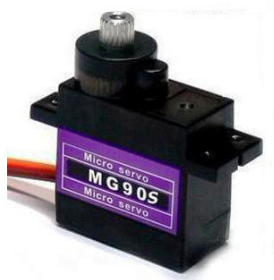
\includegraphics[height=2in]{Servo_Motor.png}
\hfill
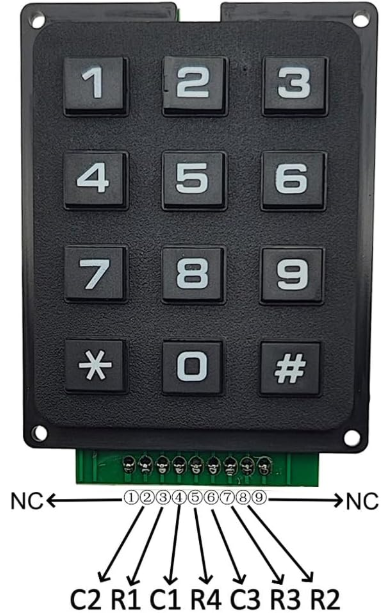
\includegraphics[height=2.5in]{keypad.png}
\hfill
\leftskip 0in \rightskip 0in

\speakernotes{<<SPEAKER\_1>>}{%
<<Word-for-word outline speech here. Mention what each speaker will cover.>>
}

\newpage

%%%%%%%%%%%%%%%%%%%%%%%%%%%%%%%%%%%%%%%%%%%%%%%%%%%%%%%%%%%%
% SLIDE 3 — FSM Diagram
% SPEAKER: Santiago
%%%%%%%%%%%%%%%%%%%%%%%%%%%%%%%%%%%%%%%%%%%%%%%%%%%%%%%%%%%%
\slideheader{Function State Machine Diagram}{Santiago}

\leftskip 0.5in \rightskip 0.7in
\vspace{0.15in}

\begin{multicols}{2}
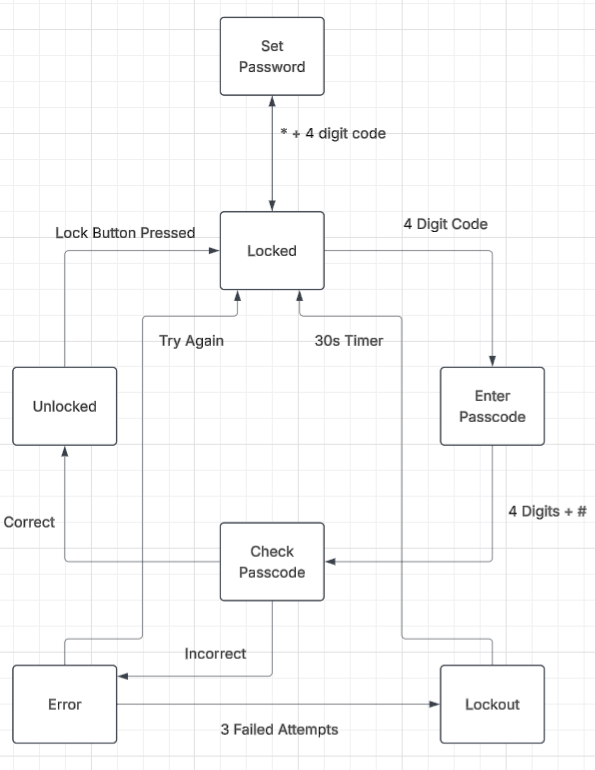
\includegraphics[height=6in,width = 4.5in]{FSM Diagram.png}

\columnbreak

\textbf{FSM Diagram States}
\begin{itemize}
  \item Locked $->$ Pass code Storage  
  \item Locked $->$ Pass code $->$ Verify $->$ Success/Error
  \item Error $->$ Lockout
\end{itemize}
\end{multicols}

\leftskip 0in \rightskip 0in

\newpage
%%%%%%%%%%%%%%%%%%%%%%%%%%%%%%%%%%%%%%%%%%%%%%%%%%%%%%%%%%%%
% SLIDE 4 — Door Design
% SPEAKER: Jacob
%%%%%%%%%%%%%%%%%%%%%%%%%%%%%%%%%%%%%%%%%%%%%%%%%%%%%%%%%%%%
\slideheader{Door Design}{Jacob}

\vspace{0.2in}

\begin{figure}[H]
    \centering
    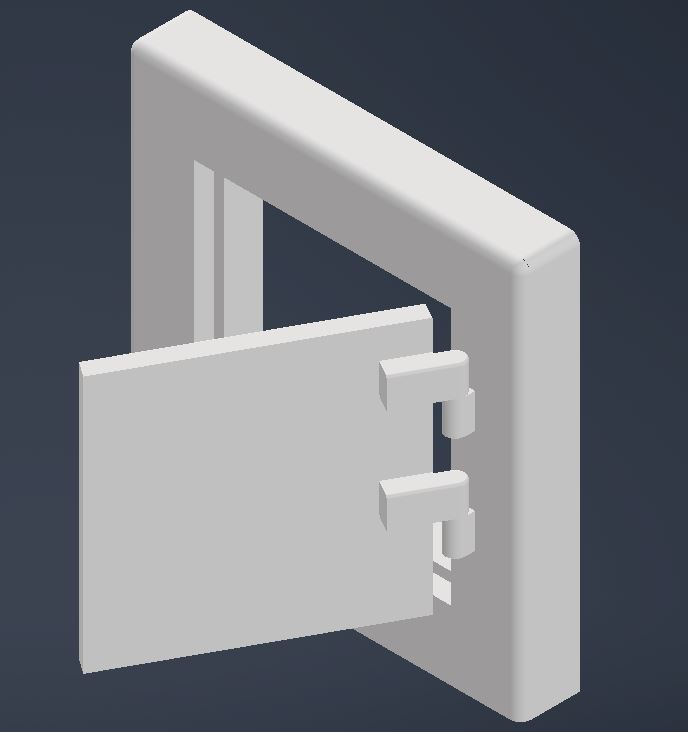
\includegraphics[width=3in]{Electronic Door Design.JPG}
    \caption{Door Design}
    \label{fig:door-design}
\end{figure}
\begin{itemize}
  \item Simple assembly of frame and door, made on Inventor AutoCAD
  \end{itemize}
\speakernotes{<<SPEAKER\_1>>}{%
<<Word-for-word outline speech here. Mention what each speaker will cover.>>
}

\newpage

%%%%%%%%%%%%%%%%%%%%%%%%%%%%%%%%%%%%%%%%%%%%%%%%%%%%%%%%%%%%
% SLIDE 4 — Theory (Part 1)
% SPEAKER: <<SPEAKER_3>>
%%%%%%%%%%%%%%%%%%%%%%%%%%%%%%%%%%%%%%%%%%%%%%%%%%%%%%%%%%%%
\slideheader{<<Theory Title 1>>}{Theory}

\leftskip 0.7in \rightskip 0.7in
\vspace{0.1in}

% <<Insert equations and bullet points for the first theory topic.>>

\leftskip 0in \rightskip 0in

\speakernotes{<<SPEAKER\_3>>}{%
<<Word-for-word theory speech here.>>
}

\newpage

%%%%%%%%%%%%%%%%%%%%%%%%%%%%%%%%%%%%%%%%%%%%%%%%%%%%%%%%%%%%
% SLIDE 5 — Theory (Part 2)
% SPEAKER: <<SPEAKER_3>>
%%%%%%%%%%%%%%%%%%%%%%%%%%%%%%%%%%%%%%%%%%%%%%%%%%%%%%%%%%%%
\slideheader{<<Theory Title 2>>}{Theory}

\leftskip 0.7in \rightskip 0.7in
\vspace{0.1in}

% <<Insert equations and bullet points for the second theory topic.>>

\leftskip 0in \rightskip 0in

\speakernotes{<<SPEAKER\_3>>}{%
<<Word-for-word theory speech here.>>
}

\newpage

%%%%%%%%%%%%%%%%%%%%%%%%%%%%%%%%%%%%%%%%%%%%%%%%%%%%%%%%%%%%
% SLIDE 6 — Problem Definition
% SPEAKER: <<SPEAKER_4>>
%%%%%%%%%%%%%%%%%%%%%%%%%%%%%%%%%%%%%%%%%%%%%%%%%%%%%%%%%%%%
\slideheader{Problem: <<Problem Title>>}{<<Application>>}

\leftskip 0.7in \rightskip 0.7in
\vspace{0.05in}

\begin{multicols}{2}
\textbf{<<Scenario description>>}

% <<Equations, data tables, or diagrams>>

\columnbreak

\textbf{Pipeline:}
\begin{enumerate}
  \item <<Step 1>>
  \item <<Step 2>>
  \item <<Step 3>>
\end{enumerate}
\end{multicols}

\leftskip 0in \rightskip 0in

\speakernotes{<<SPEAKER\_4>>}{%
<<Word-for-word problem-definition speech here.>>
}

\newpage

%%%%%%%%%%%%%%%%%%%%%%%%%%%%%%%%%%%%%%%%%%%%%%%%%%%%%%%%%%%%
% SLIDE 7 — Key Formula / Matrix Calculation
% SPEAKER: <<SPEAKER_5>>
%%%%%%%%%%%%%%%%%%%%%%%%%%%%%%%%%%%%%%%%%%%%%%%%%%%%%%%%%%%%
\slideheader{<<Formula / Matrix Title>>}{<<Subtopic>>}

\leftskip 0.7in \rightskip 0.7in
\vspace{0.1in}

% <<Insert the core mathematical derivation or matrix equation.>>

\leftskip 0in \rightskip 0in

\speakernotes{<<SPEAKER\_5>>}{%
<<Word-for-word formula explanation speech here.>>
}

\newpage

%%%%%%%%%%%%%%%%%%%%%%%%%%%%%%%%%%%%%%%%%%%%%%%%%%%%%%%%%%%%
% SLIDE 8 — Implementation (Part 1)
% SPEAKER: <<SPEAKER_6>>
%%%%%%%%%%%%%%%%%%%%%%%%%%%%%%%%%%%%%%%%%%%%%%%%%%%%%%%%%%%%
\slideheader{Implementation: <<Method Name(s)>>}{}

\leftskip 0.7in \rightskip 0.7in
\vspace{0.05in}

\begin{lstlisting}
# <<Paste key code from lib/tools.py>>
\end{lstlisting}

\leftskip 0in \rightskip 0in

\speakernotes{<<SPEAKER\_6>>}{%
<<Word-for-word code walkthrough speech here.>>
}

\newpage

%%%%%%%%%%%%%%%%%%%%%%%%%%%%%%%%%%%%%%%%%%%%%%%%%%%%%%%%%%%%
% SLIDE 9 — Implementation (Part 2)
% SPEAKER: <<SPEAKER_6>>
%%%%%%%%%%%%%%%%%%%%%%%%%%%%%%%%%%%%%%%%%%%%%%%%%%%%%%%%%%%%
\slideheader{Implementation: <<Method Name(s)>>}{}

\leftskip 0.7in \rightskip 0.7in
\vspace{0.05in}

\begin{lstlisting}
# <<Paste additional code>>
\end{lstlisting}

\leftskip 0in \rightskip 0in

\speakernotes{<<SPEAKER\_6>>}{%
<<Word-for-word code walkthrough speech (cont.) here.>>
}

\newpage

%%%%%%%%%%%%%%%%%%%%%%%%%%%%%%%%%%%%%%%%%%%%%%%%%%%%%%%%%%%%
% SLIDE 10 — Implementation (Part 3) / Demo
% SPEAKER: <<SPEAKER_7>>
%%%%%%%%%%%%%%%%%%%%%%%%%%%%%%%%%%%%%%%%%%%%%%%%%%%%%%%%%%%%
\slideheader{Implementation: <<Additional Code or Demo>>}{}

\leftskip 0.7in \rightskip 0.7in
\vspace{0.05in}

\begin{lstlisting}
# <<Paste additional code or demo pipeline>>
\end{lstlisting}

\leftskip 0in \rightskip 0in

\speakernotes{<<SPEAKER\_7>>}{%
<<Word-for-word speech. Include [DEMO CUE] markers if running a live demo.>>
}

\newpage

%%%%%%%%%%%%%%%%%%%%%%%%%%%%%%%%%%%%%%%%%%%%%%%%%%%%%%%%%%%%
% SLIDE 11 — Live Demo (if applicable)
% SPEAKER: <<SPEAKER_4>>
%%%%%%%%%%%%%%%%%%%%%%%%%%%%%%%%%%%%%%%%%%%%%%%%%%%%%%%%%%%%
\slideheader{Live Demo (<<demo\_script.py>>)}{Demo}

\leftskip 0.7in \rightskip 0.7in
\vspace{0.1in}

\begin{multicols}{2}
\textbf{Pipeline:}
\begin{enumerate}
  \item <<Step 1>>
  \item <<Step 2>>
  \item <<Step 3>>
\end{enumerate}

\columnbreak

\textbf{Key Settings:}
\begin{itemize}
  \item <<Parameter 1>>
  \item <<Parameter 2>>
\end{itemize}
\end{multicols}

\leftskip 0in \rightskip 0in

\speakernotes{<<SPEAKER\_4>>}{%
<<Word-for-word demo speech.  Include [DEMO CUE: ...] markers.>>
}

\newpage

%%%%%%%%%%%%%%%%%%%%%%%%%%%%%%%%%%%%%%%%%%%%%%%%%%%%%%%%%%%%
% SLIDE 12 — Results (Part 1)
% SPEAKER: <<SPEAKER_1>>
%%%%%%%%%%%%%%%%%%%%%%%%%%%%%%%%%%%%%%%%%%%%%%%%%%%%%%%%%%%%
\slideheader{Results: <<Result Title 1>>}{Results}

\leftskip 0.7in \rightskip 0.7in
\vspace{0.05in}

\begin{center}
\includegraphics[width=0.70\textwidth]{<<unitNN_plot1.png>>}
\end{center}

\begin{itemize}
  \item <<Observation 1>>
  \item <<Observation 2>>
\end{itemize}

\leftskip 0in \rightskip 0in

\speakernotes{<<SPEAKER\_1>>}{%
<<Word-for-word results discussion here.>>
}

\newpage

%%%%%%%%%%%%%%%%%%%%%%%%%%%%%%%%%%%%%%%%%%%%%%%%%%%%%%%%%%%%
% SLIDE 13 — Results (Part 2)
% SPEAKER: <<SPEAKER_2>>
%%%%%%%%%%%%%%%%%%%%%%%%%%%%%%%%%%%%%%%%%%%%%%%%%%%%%%%%%%%%
\slideheader{Results: <<Result Title 2>>}{Results}

\leftskip 0.7in \rightskip 0.7in
\vspace{0.05in}

\begin{center}
\includegraphics[width=0.92\textwidth]{<<unitNN_plot2.png>>}
\end{center}

\begin{itemize}
  \item <<Observation 1>>
  \item <<Observation 2>>
\end{itemize}

\leftskip 0in \rightskip 0in

\speakernotes{<<SPEAKER\_2>>}{%
<<Word-for-word results discussion here.>>
}

\newpage

%%%%%%%%%%%%%%%%%%%%%%%%%%%%%%%%%%%%%%%%%%%%%%%%%%%%%%%%%%%%
% SLIDE 14 — Comparison Table
% SPEAKER: <<SPEAKER_5>>
%%%%%%%%%%%%%%%%%%%%%%%%%%%%%%%%%%%%%%%%%%%%%%%%%%%%%%%%%%%%
\slideheader{Door Design}{Jacob}

\vspace{0.2in}

\begin{itemize}
\item INSERT COMPLETED TIMELINE
\begin{itemize}
  \item Remaining work to completed project
  \end{itemize}
\speakernotes{<<SPEAKER\_1>>}{%
<<Word-for-word outline speech here. Mention what each speaker will cover.>>
}

\newpage

%%%%%%%%%%%%%%%%%%%%%%%%%%%%%%%%%%%%%%%%%%%%%%%%%%%%%%%%%%%%
% SLIDE 15 — Discussion and Conclusion
% SPEAKER: <<SPEAKER_7>>
%%%%%%%%%%%%%%%%%%%%%%%%%%%%%%%%%%%%%%%%%%%%%%%%%%%%%%%%%%%%
\slideheader{Discussion and Conclusion}{}

\leftskip 0.7in \rightskip 0.7in
\vspace{0.05in}

\begin{multicols}{2}
\textbf{Key Findings}
\begin{itemize}
  \item <<Finding 1>>
  \item <<Finding 2>>
  \item <<Finding 3>>
\end{itemize}

\columnbreak

\textbf{Conclusion}
\begin{itemize}
  \item <<Conclusion 1>>
  \item <<Conclusion 2>>
  \item <<Conclusion 3>>
\end{itemize}
\end{multicols}

\leftskip 0in \rightskip 0in

\speakernotes{<<SPEAKER\_7>>}{%
<<Word-for-word conclusion speech here. End with ``Thank you ... any questions?''>>
}

\end{huge}
\end{document}
